% ==============================================================================
% This file is part of the "LaTeX template for writing the Final Degree Work
% report". It has been developed to aid the students of the Bachelor's Degree in
% Video Game Design and Development at the Jaume I University.
%
% (c) 2019 Sergio Barrachina Mir and José Vte. Martí Avilés
%
% The template can be used and distributed under the next license:
%  Creative Commons Attribution-NonCommercial-ShareAlike (CC BY-NC-SA)
%  http://creativecommons.org/licenses/by-nc-sa/3.0/
%  http://creativecommons.org/licenses/by-nc-sa/3.0/legalcode
%
% Atom editor configuration follows:
% !TEX root = ./report.tex
% !TeX spellcheck = en-US
% ==============================================================================

\chapter{Work Development and Results}

\minitoc{}

\bigskip{}

In this section, we will detail the development of the project starting from the game creation, and then describing each step of increased complexity of the behaviour to imitate, as well as the results obtained in each step.

\section{Game Development}

The game environment needs to include the ML Agents' classes (Agent and Academy) to train and play the game using the network. The game structure is the one shown in section ~\ref{sec:system_design}.

The camera has an NPC and a trained AI attached. One of them controls its movement automatically, and they can be changed in play time. Both of these classes have getters to 3 variables that correspond to the possible movements: mouse X movement, mouse Y movement and mouse click, which are used to rotate and shoot.

The Spawner creates randomly and saves references of black planes in the scene, which correspond to the enemies.

To end with, a Debug Canvas has been added as interface, which draws lines with the movements made and the ones expected by the neural network. This allows to see how well the neural network is training.

\section{Reactive Behaviors}

The first human behavior we would analize is reactions, which can be defined as ``sudden changes produced by a stimulus''. To model this behavior, we created a Bot with the following requirements:

\begin{itemize}
 \item While not seeing any target, it moves to the left uniformly
 \item When a target enters the screen, it reacts moving fast towards its center, then continues moving as normal
\end{itemize}

At this first step, the bot will only move in the Y axis, and it will be considered that is always clicking (so the targets would be destroyed whenever the sight touches them).

In the following subsections, some training related issues will be taken into account. At first, we will train our models using Proximal Policy Optimization (PPO)~\cite{ppopolicy}.

\subsection{Unnecessary actions}
It is important not to add more actions than needed, since they would slow down the training process considerably. Even though the agent can move in X and Y and perform clicks, since the bot only moves using the Y axis any other action would add much noise to the agent. 

That is caused because when training the agent is overfitted with demonstrations with Y movements of exactly 0, and when that AI is playing any slight up or down movement would go inside untrained cases, and then causing unexpected behaviors.

Therefore, in this case the neural network would only have 1 action output.

\subsection{Rewards based in tolerable range}

\begin{wrapfigure}{r}{0.35\textwidth}
    \centering
    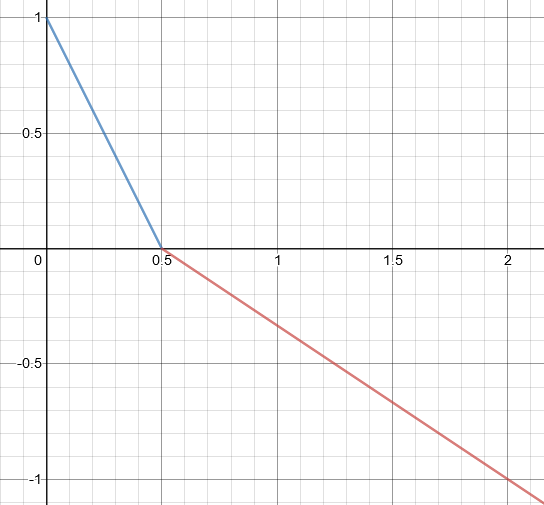
\includegraphics[width=0.35\textwidth]{img/rewTR.png}
		\caption{Rewards based in tolerable range.}
		\label{fig:trange}
\end{wrapfigure}

Our first reward approach is based in tolerable ranges. This consists in giving positive rewards when the distance between the guess and the real move is less than the tolerable range:

-The maximum reward is given (1) if it the distance is exactly 0

-A reward of -1 is given when the distance is 2, which is the maximum distance possible (NPC moving at maximum speed in one direction and the AI in the opposite direction).

In Figure~\ref{fig:trange}, you can see the reward function with tolerable range = 0.5. In our trainings, tolerable range was between 0.05 and 0.1: lower tolerable ranges caused the training to become unstable because it only got negative rewards, and higher tolerable range

Models trained using this rewards are not very time-efficient. If the tolerable range is too big (the agent receives positive rewards easily), the model doesn't fit the movement; if it is too small (receives negative rewards), the agent tends to stay only in the average movement, and doesn't react at all. That happens because the average is the point with biggest chance of reward (the agent is only punished when an impulse occurs). 

Curriculum learning~\footnote{Curriculum learning is a technique provided by ML Agents to train complex behaviors with consecutive lessons that increase in difficulty. That way, when the agent learns one task it goes on to the next lesson.} does not improve the training performance since with the initial less exigent punishments, the neural network learns much slower than with higher ones.

Figure~\ref{fig:graphTR} shows some of the success cases. From left to right, the first image shows how the neural network model adapts to the idle movement and the impulses, after 180000 training steps (4100s). The middle image displays an imperfect behavior of the same model when successive impulses occur. The right image is the same model trained longer time (10000s, 435000 steps), and how it tends to excessively smooth its impulsive movements. The causes of these two problems (successive impulses and smoothing) are discussed in section~\ref{sec:determ}.
\begin{figure}[h]
  \centering
		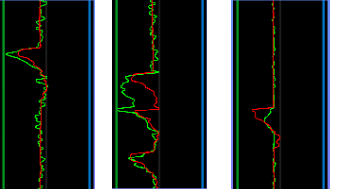
\includegraphics[width=.9\textwidth]{img/graphsTR.png}
  \caption{Bot movement (red) and neural network movement (green)}
  \label{fig:graphTR}
\end{figure}

\subsection{Determinism of the behavior}
\label{sec:determ}

Since at this point the neural network does not receive past events as input (neither moves or images), the movements performed by the bot have to be deterministic in order to train correctly: that is, given a frame, the bot would react with the exact same move every time (in the impulses, the default movement has a bit of noise in it). However, by how the bot was made it always took as objective the first image that it had seen, until destroyed.

In some special cases, when a new target spawns nearer to the sight than the current objective, the bot would not change the target order, and so it would behave differently depending on the context, as you can see in figure~\ref{fig:graphTR}. These repeated events cause the neural network to confuse when multiple targets are on screen, and if trained longer, it tends to do smaller impulses until only moving in the average move.

\begin{figure}[h]
  \centering
		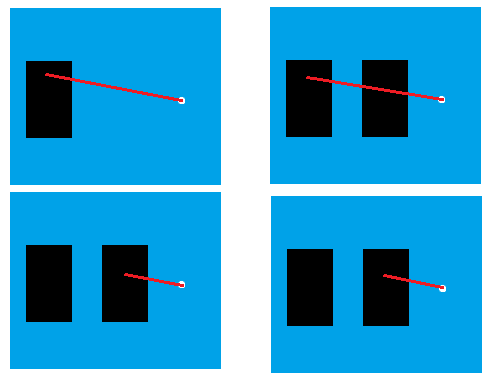
\includegraphics[width=.9\textwidth]{img/exampleDet.png}
  \caption{2 situations that lead to different actions with the same frame}
  \label{fig:graphTR}
\end{figure}

This issue is solved by making the bot behavior deterministic or adding a movement memory.

\subsection{Movement memory}

In order to prepare the bot to have reaction times, 25 previous moves distributed in the last 2 seconds are added as observations. What move is added as observation is critical.

If the real bot movement is added, the bot reaches high rewards very quickly but doesn't learn to imitate the bot: that's because the neural network learns to ``mimic'' the last move made by the bot, so it has high chance of reward with only one important observation. When playing the game with the trained neural network, it would not move (in the beginning, all the previous moves are 0) until it starts moving in one or another direction at maximum speed (See Figure~\ref{fig:graphMem}). This happens when the movement starts increasing in value due to impressions in the returned action of the neural network that make it believe that it is accelerating in movement.

When using the neural network movement, it learns like before: correctly but a bit slower. However, the previous moves tend to have noise at first, and the network could learn to ignore them.

\begin{figure}[h]
  \centering
		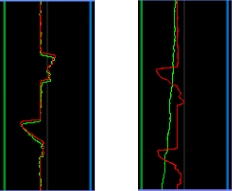
\includegraphics[width=.5\textwidth]{img/graphsMemory.png}
  \caption{A badly trained model while training (up) and playing (down)}
  \label{fig:graphMem}
\end{figure}

A better approximation would be interpolating the real move with the neural network's one: at the start, the movement added as observation in the next frames would be the NPC move. When the AI starts learning to adapt to the context (previous moves), the movement added would be an interpolation between the AI and the NPC movement (which would cause the AI to react in time), until the original AI moves are the ones added as observation. This can be made using curriculum learning: the lesson with least difficulty is the one where the AI receives past movements of the NPC as observations, and the hardest one where it receives its own movements as observation.

\subsection{Rewards based in standard deviation}
\label{sec:stdrew}

Since trained models using the methods explained in the previous sections tend to return the most common value, movements with more noise or imprecissions would not be produced correctly by the AI: when training, the AI could guess a move some units below the average of the previous moves but the NPC could have done a move the same units above the average, causing the network to be penalized, and causing the AI movement to converge to the average movement. To model these kind of noises more precisely, the actions and rewards should be changed.

In this section we propose a reward system based on standard deviations (Figure~\ref{fig:stdexample}): the relation between standard deviation, average and the actual move would determine how coherent is a move in a given context.
\begin{wrapfigure}{r}{0.2\textwidth}
    \centering
    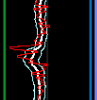
\includegraphics[width=0.2\textwidth]{img/graphSTD.png}
		\caption{Weighted average and standard deviations of an irregular movement}
		\label{fig:stdexample}
\end{wrapfigure}

The \emph{coherence} of a movement can be defined as how centered it is, in relation to the average. A movement with maximum coherence (1) would be the exact average, a movement at a standard deviation distance would have coherence 0, and movements outside of the standard deviations would be considered ``incoherent''. Then, default movement with noise would be coherent moves, and impulses would be incoherent.

To model the behavior, the agent would do 2 actions instead of one: a maximum and a minimum guess. The more precisely it encloses the real movement, the higher reward it gets; if it fails enclosing it, a punish is given.

\begin{figure}
    \centering
    \begin{subfigure}[b]{0.3\textwidth}
        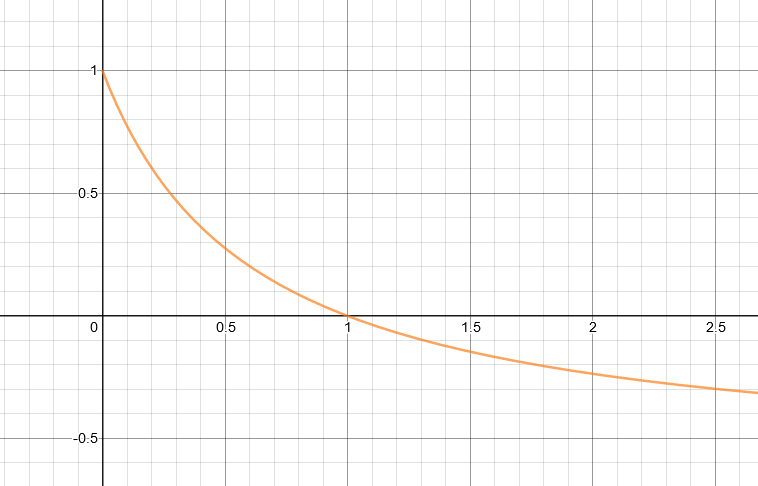
\includegraphics[width=\textwidth]{img/stdPrecision.png}
        \caption{Points by precision}
        \label{fig:prec}
    \end{subfigure}
    ~ %add desired spacing between images, e. g. ~, \quad, \qquad, \hfill etc. 
      %(or a blank line to force the subfigure onto a new line)
    \begin{subfigure}[b]{0.3\textwidth}
        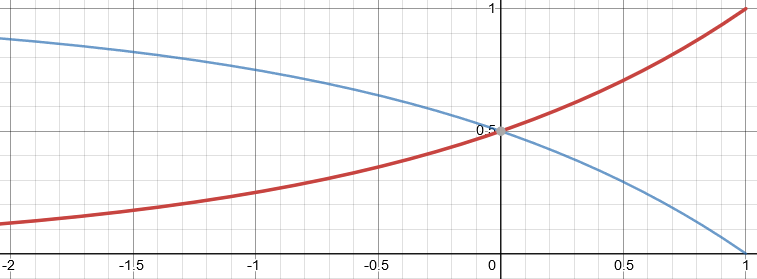
\includegraphics[width=\textwidth]{img/stdFactors.png}
        \caption{Reward and punishment factors by coherence}
        \label{fig:stdf}
    \end{subfigure}
    ~ %add desired spacing between images, e. g. ~, \quad, \qquad, \hfill etc. 
    %(or a blank line to force the subfigure onto a new line)
    \begin{subfigure}[b]{0.3\textwidth}
        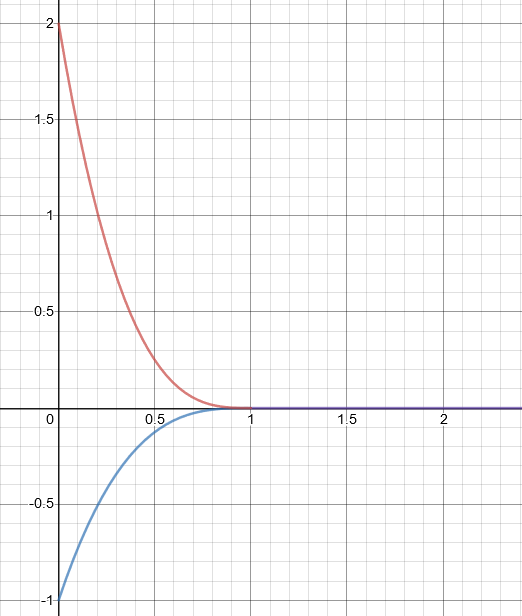
\includegraphics[width=\textwidth]{img/stdDevfactor.png}
        \caption{Deviation factor divided by Pow(2,(1-coherence)), with coherence=1}
        \label{fig:devf}
    \end{subfigure}
    \caption{Shape of the 3 parameters used for rewards}
		\label{fig:stdshapes}
\end{figure}

\begin{wrapfigure}{r}{0.2\textwidth}
    \centering
    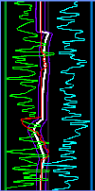
\includegraphics[width=0.2\textwidth]{img/graphsSTDrew.png}
		\caption{Trained model using SD rewards}
		\label{fig:stdrewards}
\end{wrapfigure}

Coherent moves give higher punishments if failing and smaller rewards, and incoherent moves (impulses) give high rewards. Given a maximum and minimum values (actions provided by the neural network), the real move, the average of the last 25 moves, its standard deviation and the coherence parameter explained in this section, the reward system follows these rules:

\begin{itemize}
 \item \emph{Coherence} is inversely proportional to the \emph{reward factor}, and directly proportional to the \emph{punish factor}: high coherence means lower rewards and higher punishes.
 \item A movement has higher \emph{precision} if it's centered between the maximum and minimum, and less precision if it's outside
 \item The \emph{precision} is relative to the difference between the maximum and minimum values
 \item The \emph{deviation factor} is calculated dividing the real standard deviation with the agent one (max - min)
 \item The \emph{deviation factor} is inversely proportional to the coherence
 \item All the values are clamped to avoid excessively high rewards/punishments or zero division errors
 \item The final reward is calculated multiplying \emph{precision * factor * deviation factor}
\end{itemize}

In figure~\ref{fig:stdshapes} you can see the shapes of each parameter functions, used to calculate the final reward.


In this first approach using maximum and minimum estimations, the network doesn't fit well the movement: it encloses large areas continuously (See Figure~\ref{fig:stdrewards}). That could happen because it receives less punishment by enclosing the coherent movement than by fitting and sometimes failing, and also receives rewards from incoherent movement. Thus, the neural network finds an equilibrium enclosing wide ranges to catch high rewards from incoherent moves, at the cost of getting fewer rewards from coherent moves (which were low by definition) and not exposing to any punishment from failing to encase coherent moves.

\subsection{Rewards based in movement coherence}
\label{sec:cohrew}

Since last reward system didn't make the agent learn correctly, we need to change the rewards in a way that it worries about adjusting to the predictable coherent movement while also worrying about not to miss any impulsive incoherent move.

Rewards based on movement coherence are a simplification of the reward system exposed on section ~\ref{sec:stdrew}, where coherent moves can only punish and incoherent moves can only give rewards. These motivates the agent to receive the least punishments by enclosing coherent moves, but also to take profit of potential rewards of incoherent moves. 

\begin{wrapfigure}[11]{rH}{0.4\textwidth}
    \centering
    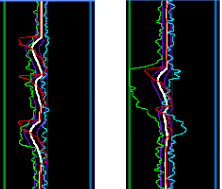
\includegraphics[width=0.4\textwidth]{img/graphsCoherence.png}
		\caption{Coherence-based models with and different learning rate: left=2e-3, right=8e-3}
		\label{fig:precisionR}
\end{wrapfigure}

The punishments in coherent moves are calculated multiplying the punish factor, the coherence (0..1) and the relative distance between standard deviations, maximum and minimum.

The rewards in incoherent moves are calculated using the reward factor, the opposite to coherence (0..N, coherence is negative) and the precision factor shown in section~\ref{sec:stdrew}.

Models trained with this system adapt better to both coherent and incoherent moves, however they need high learning rate and at least 300000 steps to see acceptable results (see Figure~\ref{fig:precisionR}). However, a learning rate higher than 1e-2 can easily lead to unstable models that don't learn at all.

\subsection{PPO hyperparameters}

To sum up, the trained models that got decent performance had the following hyperparameters (they also depend on the reward system):

\begin{center}
	\begin{tabular}{ | m{4cm} | m{2.5cm}||m{4cm} | m{2.5cm} | } 
		\hline
			batch size & 32 or 1024 & beta & 5.0e-3..8.0e-3\\ 
		\hline
			buffer size & 256 or 8196 & epsilon & 0.3\\
		\hline
			hidden units & mostly 256 & learning rate & 1.0e-4..2.0e-3\\
		\hline
			learning rate schedule & mostly linear & normalize & false\\
		\hline
			num layers & mostly 1 & num epoch & 3-5\\
		\hline
			summary freq & 1000 & time horizon & 5-256\\
		\hline
			extrinsic strength & 1.0 & extrinsic gamma & 0.8..0.9\\
		\hline
			curiosity strength (opt.) & 0.01..0.1 & curiosity gamma (opt.) & 0.8..0.99\\
		\hline
			curiosity encoding size (opt.) & 128-256 & gail strength & 0.01 (not recommended)\\
		\hline
			gail gamma & 0.95 (not rec.) & gail learning rate & 0.0005 (not rec.)\\
		\hline
			gail encoding size & 64 (not rec.) & gail use vail & true (not rec.)\\
		\hline
			gail use actions & true (not rec.) & & \\
		\hline
	\end{tabular}
\end{center}

\subsection{Training with Soft-Actor Critic (SAC)}

Soft-Actor Critic is the second reinforcement learning policy provided in ML-Agents~\cite{mlagents}. It is characterized for being more sample-efficient and can learn from past experiences. However, it also executes slower, so the time needed to train a model is very similar both with PPO and SAC. Also, its training steps can be increased more easily since the learning rate is recommended to be constant (its Q function converges naturally).

To compare new methods with SAC and PPO, we've added simple linear rewards that affect the maximum and minimum individually, in addition to rewards based in movement coherence. These give reinforcement signals when one of the lines is well positioned, even when the cummulative reward is negative. In Figure~\ref{fig:pposac} you can see a cumulative reward comparison between an agent trained with SAC and other agent trained using PPO, with rewards based in coherence (see section~\ref{sec:cohrew}): SAC converges to a higher reward than PPO with much less steps.

\begin{figure}[h]
  \centering
		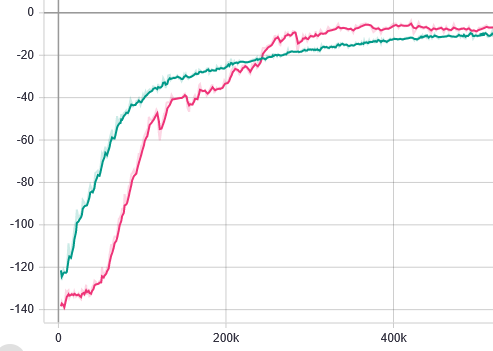
\includegraphics[width=.6\textwidth]{img/PpoSac.png}
  \caption{Total rewards of SAC (pink) and PPO (green).}
  \label{fig:pposac}
\end{figure}

As final result, Figure~\ref{fig:graphPS} shows a comparison between both trained neural networks: SAC adapts much better to impulses than PPO, even though PPO also manages to fit the real move between the two lines. However, when playing neither of them reacts correctly to targets that appear on the right side (mainly because it is an uncommon case). After the training both models still have much noise in their default movement, but it could be corrected by training longer or by rewarding the stability of both agent lines (maximum and minimum).

\begin{figure}[h]
  \centering
		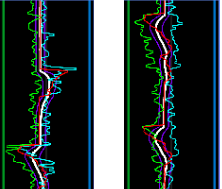
\includegraphics[width=.6\textwidth]{img/graphSacPpo.png}
  \caption{Comparison between SAC (left) and PPO (right).}
  \label{fig:graphPS}
\end{figure}

Another aspect to take into account is how both methods can be applied using GPUs to boost the training process. SAC makes better use of the GPU: by training with 3 environments in parallel the training speed doubles (being equally fast as PPO using CPU) and also improves its efficiency. PPO training using GPU and 3 environments is almost 2.5 times faster than with CPU or GPU-SAC, but is more likely to produce an application crash than any other training method (because of GPU overheating or running out of memory).

\subsection{SAC hyperparameters}

These parameters were the ones used when training with SAC:
\begin{center}
	\begin{tabular}{ | m{4cm} | m{2.5cm}||m{4cm} | m{2.5cm} | } 
		\hline
			batch size & 128 & buffer size & 200000\\ 
		\hline
			buffer init steps & 5000 & hidden units & 256\\
		\hline
			init entcoef & 1.0 & learning rate & 4.0e-4\\
		\hline
			learning rate schedule & constant & max steps & 6.0e5\\
		\hline
			memory size & 256 & normalize & true\\
		\hline
			num update & 1 & train interval & 5\\
		\hline
			num layers & 1 & time horizon & 64\\
		\hline
			sequence length & 128 & summary freq & 1000\\
		\hline
			tau & 0.005 & use recurrent & false\\
		\hline
			vis encode type & simple & pretraining strength & 0.4\\
		\hline
			pretraining steps & 20000 & extrinsic strength & 1.5\\
		\hline
			extrinsic gamma & 0.99 & curiosity strength & 0.03\\
		\hline
			curiosity gamma & 0.99 & curiosity encoding size & 128\\
		\hline
			gail strength & 0.03 & gail gamma & 0.99\\
		\hline
			gail encoding size & 128 & use actions & true\\
		\hline
	\end{tabular}
\end{center}